\documentclass[logo,reportComp]{thesis}
\usepackage[cpp,pseudo]{mypackage}

\title{操作系统原理实验报告}
\subtitle{实验十一:多终端}
\school{数据科学与计算机学院}
\author{陈鸿峥}
\classname{17大数据与人工智能}
\stunum{17341015}
\headercontext{操作系统原理实验报告}
% \authorremark{本实验报告用\LaTeX撰写,创建时间:\builddate\today}

\begin{document}

\maketitle

\section{实验目的}
\begin{itemize}
	\item 学习设备管理的方法,掌握其键盘和显示的驱动
	\item 扩展 MyOS 的内核,利用虚拟键盘和显示器的方法,实现进程的输入和输出的独立,即多终端
\end{itemize}

\section{实验要求}
% 实验目的和实验要求由老师提供实验项目文档中获取
\begin{enumerate}
	\item 禁止使用 BIOS 的键盘中断和屏幕输出调用,在 MyOS 实现自己的键盘输入驱动和显示器驱动。
	\item 修改和扩展 MyOS 的系统调用,实现在 C 语言中,程序格式化输入和输出在独立的终端上进行,利用\verb'CTRL+F1'、\verb'CTRL+F2'、\verb'CTRL+F3'可以切换不同的终端。
\end{enumerate}

\section{实验环境}
% 包括:硬件或虚拟机配置方法、软件工具与作用、方案的思想、相关原理、程序流程、算法和数据结构、程序关键模块,结合代码与程序中的位置进行解释。不得抄袭,否则按作弊处理。
% 实验方案包括相关基础原理、实验工具和环境、程序流程和算法思想、数据结构与程序模块功能说明,代码文档组成说明等
具体环境选择原因已在实验一报告中说明。
\begin{itemize}
	\item Windows 10系统 + Ubuntu 18.04(LTS)子系统
	\item gcc 7.3.0 + nasm 2.13.02 + GNU ld (Binutils) 2.3.0
	\item GNU Make 4.1
	\item Oracle VM VirtualBox 6.0.6
	\item Bochs 2.6.9
	\item Sublime Text 3 + Visual Studio Code 1.33.1
\end{itemize}

虚拟机配置:内存4M,1.44M虚拟软盘引导,1.44M虚拟硬盘。

\section{实验方案}
% 包括:主要工具安装使用过程及截图结果、程序过程中的操作步骤、测试数据、输入及输出说明、遇到的问题及解决情况、关键功能或操作的截图结果。不得抄袭,否则按作弊处理。
{\textbf{\textcolor{red}{本次实验继续沿用实验六保护模式的操作系统。用户程序都以ELF文件格式读入,并且在用户态(ring 3)下执行。}}}

多终端看上去内容很少,但实际上要修改的内容还是挺多的,涉及到进程和文件系统的处理。

\subsection{多终端保护}
在\verb'terminal.h'中创建终端的结构体,将\textbf{显示器、光标、文件路径}全部记录下来。
同时创建一个\verb'terminal_list'统一进行管理。
\begin{lstlisting}
typedef struct terminal
{
	int num;
	int cursor;
	char buf[VIDEO_SIZE];
	char path[50];
	int dir;

} terminal_t;
static terminal_t terminal_list[MAX_TERMINAL];
\end{lstlisting}

还需要在进程中添加一个\verb'terminal'项,用来管理进程是在哪个终端创建的,则该进程只会在那个终端输出。

为辨别不同的切换情况,这里我采用了两个指针,如下
\begin{lstlisting}
terminal_t *curr_terminal, *tmp_terminal;
\end{lstlisting}
前一个指针记录当前终端,也就是显示的终端;后一个指针记录当前进程对应的中断,即该进程要输出的终端号。
当切换进程时,切换的是\verb'tmp_terminal',而键盘切换的则是\verb'curr_terminal'。

而输出到哪里也主要依据这两个终端号是否相同,通过下列函数获取对应的输出地址。
\begin{lstlisting}
uintptr_t get_terminal_buf_addr()
{
	if (curr_terminal->num == tmp_terminal->num)
		return VIDEO_ADDRESS;
	else
		return (uintptr_t)&tmp_terminal->buf;
}
\end{lstlisting}

实际上终端的切换跟进程的切换是类似的,需要保护现场、恢复现场。
\begin{lstlisting}
void change_terminal(int new_ter)
{
	disable();
	memcpy((void*)curr_terminal->buf,(void*)VIDEO_ADDRESS,VIDEO_SIZE);
	curr_terminal->cursor = get_cursor();
	get_curr_path(curr_terminal->path);
	curr_terminal->dir = get_curr_dir();
	if (get_proc() == NULL)
		curr_terminal = tmp_terminal = &terminal_list[new_ter];
	else
		curr_terminal = &terminal_list[new_ter];
	clear_screen();
	memcpy((void*)VIDEO_ADDRESS,(void*)curr_terminal->buf,VIDEO_SIZE);
	set_cursor(curr_terminal->cursor);
	set_curr_path(curr_terminal->path);
	set_curr_dir(curr_terminal->dir);
	enable();
}
\end{lstlisting}

\subsection{键盘中断}
由于在实验六时进入保护模式,键盘中断已经是自己写的,故只需在原有基础上对功能键进行判断即可。
\begin{lstlisting}
void keyboard_handler_main(void)
{
	unsigned char status;
	unsigned char scancode;

	/* write EOI */
	port_byte_out(0x20, 0x20);

	status = port_byte_in(KEYBOARD_STATUS_PORT);
	/* Lowest bit of status will be set if buffer is not empty */
	if (status & 0x01) {
		scancode = port_byte_in(KEYBOARD_DATA_PORT);
		if (scancode < 0)
			return;
		if (scancode & 0x80) {
			if (scancode - 0x80 == KEY_CTRL)
				__ctrl = false;
		} else {
			if (scancode == KEY_CTRL)
				__ctrl = true;
			else if (__ctrl && scancode == KEY_F1)
				change_terminal(0);
			else if (__ctrl && scancode == KEY_F2)
				change_terminal(1);
			else if (__ctrl && scancode == KEY_F3)
				change_terminal(2);
			else {
				char ascii = asccode[(unsigned char) scancode][0];
				kb_char = ascii;
			}
		}
	}
}
\end{lstlisting}


\section{实验结果}
多终端的效果如图\ref{fig:terminal}和图\ref{fig:terminal-after}所示,由\verb'CHZOS'后的标号可以看见是几号终端。
\begin{figure}[H]
\centering
\begin{tabular}{cc}
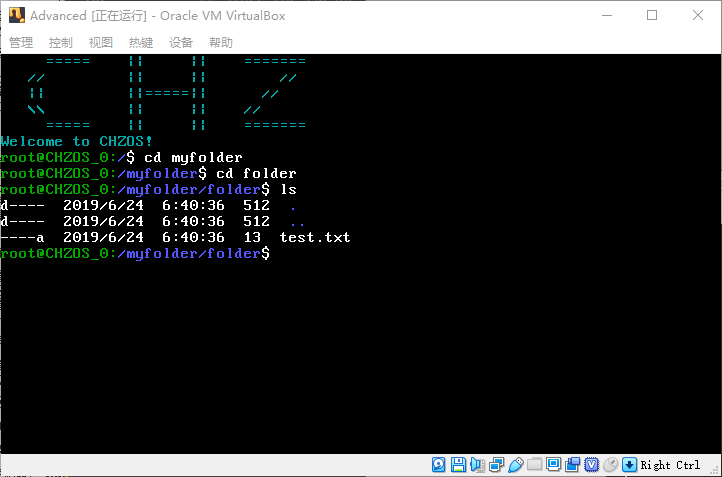
\includegraphics[width=0.5\linewidth]{fig/term_1.png}&
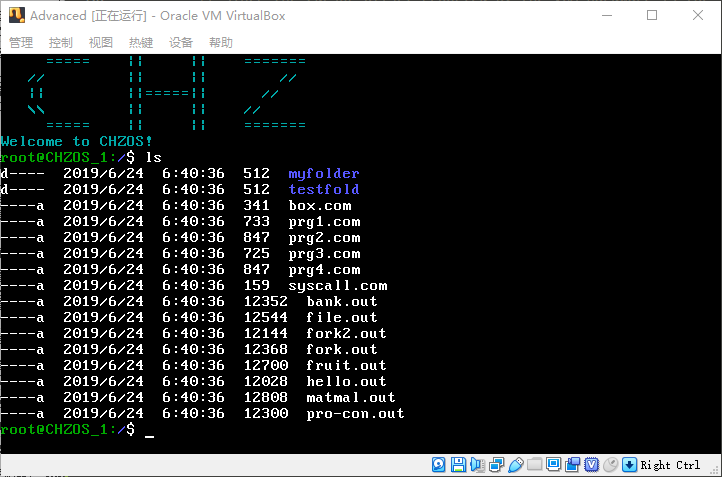
\includegraphics[width=0.5\linewidth]{fig/term_2.png}\\
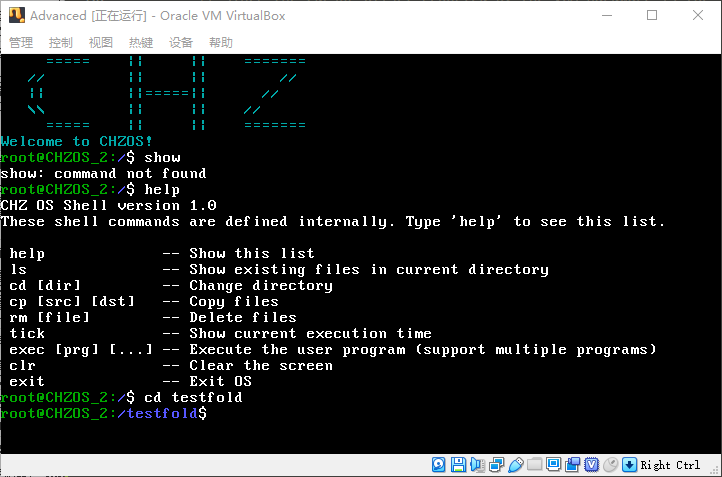
\includegraphics[width=0.5\linewidth]{fig/term_3.png}
\end{tabular}
\caption{三个终端初始状态,注意它们分别处在不同的目录。由于保护了目录信息,故切换终端不会导致目录出错。}
\label{fig:terminal}
\end{figure}

\begin{figure}[H]
\centering
\begin{tabular}{cc}
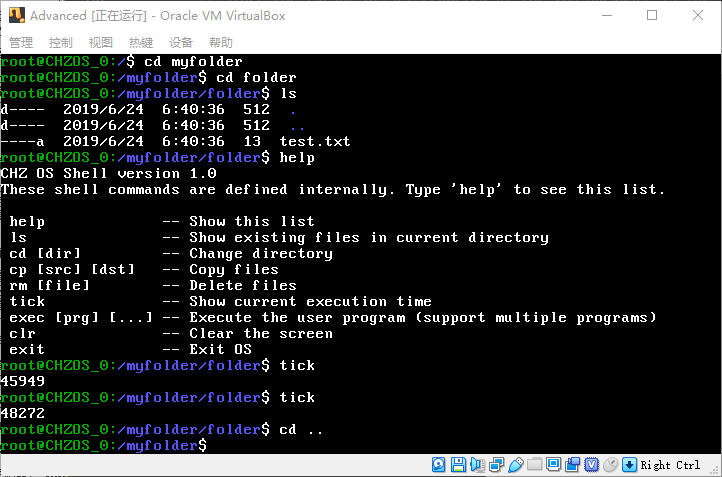
\includegraphics[width=0.5\linewidth]{fig/term_1-after.png}&
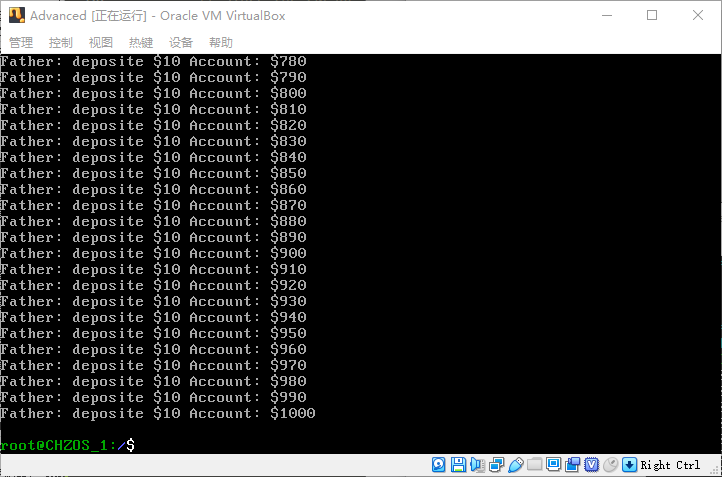
\includegraphics[width=0.5\linewidth]{fig/term_2-after.png}\\
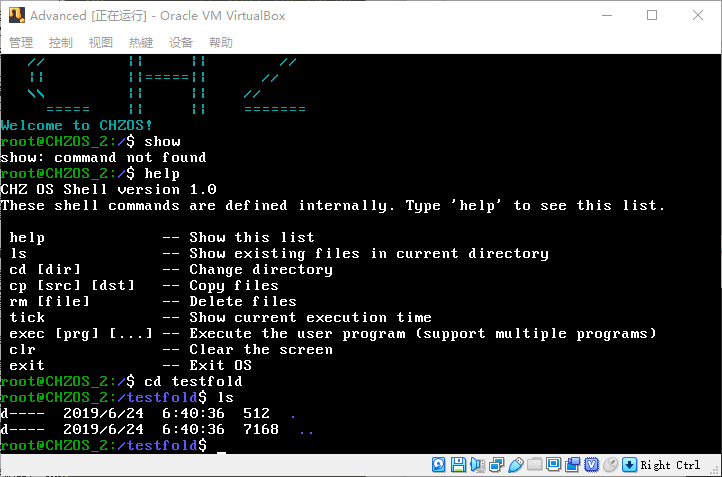
\includegraphics[width=0.5\linewidth]{fig/term_3-after.png}
\end{tabular}
\caption{在第二个终端运行进程后,再在其他终端进行操作(如执行其他进程、展示文件列表、计时等),发现操作系统能够正常运行,并且不会产生错误。}
\label{fig:terminal-after}
\end{figure}

\section{实验总结}
% 每人必需写一段,文字不少于500字,可以写心得体会、问题讨论与思考、新的设想、感言总结或提出建议等等。不得抄袭,否则按作弊处理。
本次实验是操作系统的最后一次实验,虽然不是很难,但依然要修改的东西比较多。
由于没有可以参考的代码,故所有的实现方法都是自己想的。
最终想到用两个不同的指针实现多终端的切换,并实施出来验证了自己的想法,还是挺开心的。
一开始没考虑周全,只考虑了进程切换的情况,经过调试发现文件系统也会与多终端有关,故要对文件系统也提供多终端支持,否则更换终端之后文件目录还没有换,这会导致文件索引时出现大问题。

总的来说,一个学期将操作系统11个实验完整实施下来,学到了非常非常多的东西。
老师上课一直调侃说我们总会说\verb'I hate OS!',但于我而言,操作系统的实验真是一个\textbf{痛并快乐着}的过程。
这一个学期下来不知上网搜索了多少资料,阅读了多少英文文献。
看过几千页的Intel CPU说明书,也看过人家真实十几万行的操作系统代码。
光是看懂其实就有一定难度,毕竟资料并不一定全面,还要将其完整实施出来更是难上加难。
我一直跟自己说,全世界只有你懂你自己的操作系统,所以遇到问题也只有我自己能够解决。
就是这样,我跪着也要把操作系统给做完,因为只有我自己懂它。

这其中的收获是巨大的,一方面对操作系统理论有了十分透彻的理解,知道这些理论到底怎么指导实际的实施;另一方面则是对各种工具的使用更加灵活,如C和x86汇编的编写,Makefile及Windows 10子系统WSL的使用等等。
其实顺带着也把编译原理也给稍微学了一下,因为常常要看C语言编写的程序转换成汇编的结果,还要理解诸如函数堆栈等调用法则,这些其实都跟编译密切相关。

我也跟信计的同学讨论过,他们使用UCore进行实验,到底是比我们更难还是更简单。
经过一个学期的实践,我确信我们的方式代码量更大,学到的东西也更多。
我看过UCore的代码,基本的函数都已经封装好了,学生只用编写对应实验中几个函数即可,这其实与算法设计又有什么区别呢?
但操作系统不是算法设计,它是一个\textbf{系统},如何做好封装、设计简单易用的接口,如何将各个部分有机地耦合在一起,如何组合才能使性能达到最优,这些问题都是系统设计者需要思考的,而仅仅是函数的编写相当于把这些部分都抹除了,更加细节的东西不清楚,而只知大概不知全貌。
因此,我特别感谢老师能给我们一次从下到上的操作系统游览之旅,这一趟下来真是获益匪浅。

图\ref{fig:git}清晰展示了我这学期肝保护模式操作系统的状况,中间有段时间在忙其他科目的大作业,因此就停滞了一段时间。
待到期末才终于挤出点时间来,可以好好将我的操作系统彻底完善。
最终新增代码量破万,着实算是一个中型的项目了。
\begin{figure}[H]
\centering
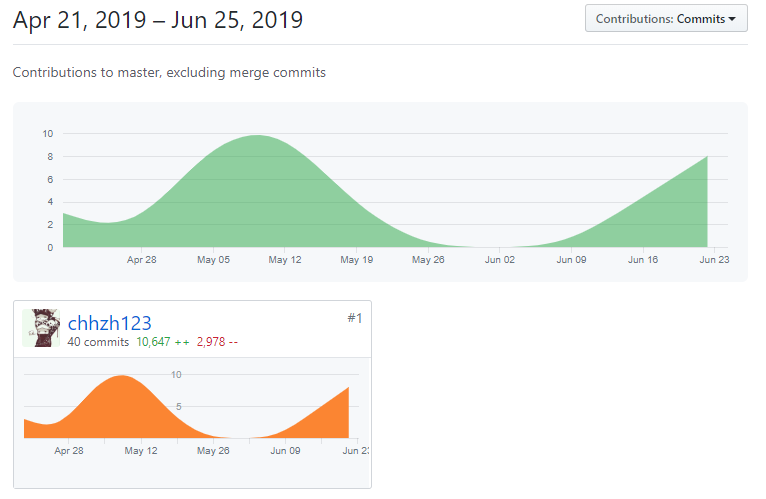
\includegraphics[width=0.8\linewidth]{fig/github.png}
\caption{Git提交记录}
\label{fig:git}
\end{figure}

最后的最后,为本学期操作系统实验完结撒花,希望我以后还能保持这样的热情去挑战更为困难的难关!

\section{参考资料}
\textbf{操作系统实现完整资料:}
\begin{enumerate}
	\item OS Development Series, \url{http://www.brokenthorn.com/Resources/OSDevIndex.html}
	\item Roll your own toy UNIX-clone OS, \url{http://www.jamesmolloy.co.uk/tutorial_html/}
	\item The little book about OS development, \url{http://littleosbook.github.io/}
	\item Writing a Simple Operating System from Scratch, \url{http://www.cs.bham.ac.uk/~exr/lectures/opsys/10_11/lectures/os-dev.pdf}
	\item Intel$^{\textregistered}$ 64 and IA-32 Architectures Software Developer's Manual
	\item UCore OS Lab, \url{https://github.com/chyyuu/ucore_os_lab}
	\item CMU CS 15-410, Operating System Design and Implementation, \url{https://www.cs.cmu.edu/~410/}
	\item 李忠,王晓波,余洁,《x86汇编语言-从实模式到保护模式》,电子工业出版社,2013
\end{enumerate}

\appendix
\appendixconfig
\section{程序清单}
\subsection{内核核心代码}
\begin{center}
\begin{tabular}{|c|l|l|}\hline
\textbf{序号} & \textbf{文件} & \textbf{描述} \\\hline
1 & \verb'bootloader.asm' & 主引导程序\\\hline
2 & \verb'kernel_entry.asm' & 内核汇编入口程序\\\hline
3 & \verb'kernel.c' & 内核C入口程序\\\hline
4 & \verb'Makefile' & 自动编译指令文件\\\hline
5 & \verb'bootflpy.img' & 引导程序/内核软盘\\\hline
6 & \verb'mydisk.hdd' & 虚拟硬盘\\\hline
7 & \verb'bochsrc.bxrc' & Bochs配置文件\\\hline
\end{tabular}
\end{center}

\subsection{内核头文件}
\begin{center}
\begin{tabular}{|c|l|l|}\hline
\textbf{序号} & \textbf{文件} & \textbf{描述} \\\hline
1 & \verb'disk_load.inc' & BIOS读取磁盘\\\hline
2 & \verb'show.inc' & 常用汇编字符显示\\\hline
3 & \verb'gdt.inc' & 汇编全局描述符表\\\hline
4 & \verb'gdt.h' & C全局描述符表\\\hline
5 & \verb'idt.h' & 中断描述符表\\\hline
6 & \verb'hal.h' & 硬件抽象层\\\hline
6.1 & \verb'pic.h' & 可编程中断控制器\\\hline
6.2 & \verb'pit.h' & 可编程区间计时器\\\hline
6.3 & \verb'keyboard.h' & 键盘处理\\\hline
6.4 & \verb'tss.h' & 任务状态段\\\hline
6.5 & \verb'ide.h' & 硬盘读取\\\hline
7 & \verb'io.h' & I/O编程\\\hline
8 & \verb'exception.h' & 异常处理\\\hline
9 & \verb'syscall.h' & 系统调用\\\hline
10 & \verb'task.h' & 多进程设施\\\hline
11 & \verb'user.h' & 用户程序处理\\\hline
12 & \verb'terminal.h' & Shell\\\hline
13 & \verb'scancode.h' & 扫描码\\\hline
14 & \verb'stdio.h' & 标准输入输出\\\hline
15 & \verb'string.h' & 字符串处理\\\hline
16 & \verb'elf.h' & ELF文件处理\\\hline
17 & \verb'api.h' & 进程管理API\\\hline
18 & \verb'semaphore.h' & 信号量机制\\\hline
19 & \verb'systhread.h' & 线程模型\\\hline
20 & \verb'pthread.h' & 线程管理API\\\hline
21 & \verb'fat12.h' & FAT12文件系统\\\hline
22 & \verb'sysfile.h' & 虚拟文件系统\\\hline
23 & \verb'file.h' & 文件管理API\\\hline
\end{tabular}
\end{center}

\subsection{用户程序}
用户程序都放置在\verb'usr'文件夹中。
\begin{center}
\begin{tabular}{|c|l|l|}\hline
\textbf{序号} & \textbf{文件} & \textbf{描述} \\\hline
1-4 & \verb'prgX.asm' & 飞翔字符用户程序\\\hline
5 & \verb'box.asm' & 画框用户程序\\\hline
6 & \verb'sys_test.asm' & 系统中断测试\\\hline
7 & \verb'fork_test.c' & 进程分支测试\\\hline
8 & \verb'fork2.c' & 进程多分支测试\\\hline
9 & \verb'bank.c' & 银行存取款测试\\\hline
10 & \verb'fruit.c' & 父子祝福水果测试\\\hline
11 & \verb'prod_cons.c' & 消费者生产者模型测试\\\hline
12 & \verb'hello_world_thread.c' & 多线程Hello\_world测试\\\hline
13 & \verb'matmul.c' & 多线程矩阵乘法测试\\\hline
14 & \verb'file.c' & 文件读写测试\\\hline
\end{tabular}
\end{center}

\section{系统调用清单}
\label{sec:syscall}
\begin{center}
\begin{tabular}{|c|c|}\hline
\verb'int 0x80'\textbf{功能号} & \textbf{功能}\\\hline
0 & 输出OS Logo\\\hline
1 & 睡眠100ms\\\hline
10 & \verb'fork'\\\hline
11 & \verb'wait'\\\hline
12 & \verb'exit'\\\hline
13 & \verb'get_pid'\\\hline
20 & \verb'get_sem'\\\hline
21 & \verb'sem_wait'\\\hline
22 & \verb'sem_signal'\\\hline
23 & \verb'free_sem'\\\hline
100 & 返回内核Shell\\\hline
\end{tabular}
\end{center}

\begin{center}
\begin{tabular}{|c|c||c|c|}\hline
\verb'int 0x81'\textbf{功能号} & \textbf{功能} & \verb'int 0x82'\textbf{功能号} & \textbf{功能}\\\hline
0 & \verb'pthread_create' & 0 & \verb'fopen'\\\hline
1 & \verb'pthread_join' & 1 & \verb'fclose'\\\hline
2 & \verb'pthread_self' & 2 & \verb'fread'\\\hline
3 & \verb'pthread_exit' & 3 & \verb'fwrite'\\\hline
&& 4 & \verb'fgets'\\\hline
&& 5 & \verb'fputs'\\\hline
\end{tabular}
\end{center}

\end{document}

% 实验提交内容
% 实验报告:电子版(Word2003的DOC格式或PDF格式)
% 原程序文件及可执行代码程序文件
% 测试输入数据文件和输出数据文件
% 虚拟机软盘映像文件

% 基础实验项目5个和扩展实验7个
% 实验项目,迟交影响成绩评价!
% 工具与环境可由选择,开发新型工具或优化一套开发环境都可加分!
% 一系列基础实验项目必须连续完成,当前项目只能在前一个项目的基础上进行,体现出前后的进化关系,否则要被约谈,证明没有抄袭行为!
% 一个项目可提交多个改进的版本,实现新功能和个性化特征都有利于提高相应项目的成绩。
% 实验项目提交内容用winrar工具整体压缩打包,统一格式命名为:
%	<学号>+<姓名>+<实验项目号>+<版本号>.rar
%	姓名(学号)实验NvX.zip
%	实验报告、项目文件夹、映像文件
%	ftp://172.18.216.232 sysuac 下周六23:59

% 免考
% 条件:实验1~6全部评价AAAAB+B+或相当
% 最终成绩可能范围:75分以上